% Matteo Esposito
% Corso di Ingegenria degli Algoritimi
% Dicembre 2017
% Main.tex

%--------------- Package Usati ---------------%
\documentclass[10pt,a4paper,oneside]{matc3mem}
\usepackage{geometry}
\geometry{
	a4paper,
	total={170mm,257mm},
	left=10  mm,
	top=20mm,
	right=10 mm,
}
\usepackage{tikz}
\usepackage{multicol} 
\usepackage[utf8]{inputenc}
\usepackage{graphicx}
\usepackage{listings,lstautogobble}
\usepackage{xcolor}
\usepackage{graphicx}
\usepackage{wrapfig}
\usepackage[ampersand]{easylist}
\usepackage{float}
\usepackage[italian]{babel}

\definecolor{RoyalBlue}{cmyk}{1, 0.50, 0, 0}

\lstset{language=Python,
	keywordstyle=\color{RoyalBlue},
	basicstyle=\scriptsize\ttfamily,
	commentstyle=\ttfamily\itshape\color{gray},
	stringstyle=\ttfamily,
	showstringspaces=false,
	breaklines=true,
	frameround=ffff,
	frame=single,
	rulecolor=\color{black},
	autogobble=true
}
\usepackage{showexpl}
\usepackage{zlmtt}
\usepackage{fancyvrb}
\usepackage{ragged2e}
\usepackage{titling}
%----------------------------------------------%


\begin{document}

%--------------- Trick Usati ---------------%
\renewcommand\maketitlehooka{\null\mbox{}\vfill}
\renewcommand\maketitlehookd{\vfill\null}
%------------------------------------------%

%--------------- Titolo ---------------%
\author{Matteo Esposito \\ Matricola: 0238638}
\title{Relazione Progetto in Itinere I \\
	\large Corso di Ingegneria Degli Algoritmi}
\date{Dicembre 2017}
%-------------------------------------%

%--------------- Comandi Iniziali---------------%
\frontmatter
\begin{titlingpage}
\maketitle
\end{titlingpage}
\newpage
\tableofcontents
%----------------------------------------------%

%--------------- Capitoli ---------------%
\mainmatter
\chapter{Abstract}
\section{Premessa}
L'algoritmo presentato vorrebbe tentare di risolvere il problema N.2 il quale chiedeva:\\ 
\begin{center}
	\emph{"Siano   dati   due   alberi   AVL   A   e   B   tali   che   le   chiavi   di   uno   siano   tutte strettamente   minori   delle   chiavi   dell'altro.   Progettare   e   implementare   un algoritmo   che   restituisca   un   nuovo   albero   AVL   ottenuto   come concatenazione   di   A   e   B."}\\
\end{center}
L'approccio risolutivo consta dell'utilizzo di operazioni pre-esistenti, forniteci attraverso le classi e gli snipset presenti sulla pagina di GitHub del Corso, con una classe "extendedAVL" che riporta alcune funzioni il cui scopo \'e estendere ulteriormente la classe AVLDict. Il tempo di esecuzione totale nel caso peggiore risulta essere $O(log(n))$ in quanto ogni singola operazione svolta nel caso peggiore risulta essere eseguita per un tempo pari all'$O(log(n))$.
\\ \\
Il codice \'e cos\'i strutturato:
\begin{easylist}[itemize]
	& main.py: contenente essenzialmente le DEMO dell'algoritmo
	& la classe "ProjUtilities":contenente le principali classi ed il core dell'algoritmo stesso ( la funzione \emph{concatenate} )
	& la succitata classe extendedAVL 
	& tutte le librerie e classi fornite precedentemente attraverso la pagina di GitHub.
\end{easylist} 


\chapter{L'Algoritmo}
\paragraph{Attenzione:} per brevità, verr\'a trattato estensivamente nella descrizione solo il caso in cui B sia pi\'u alto di A, il caso inverso, comunque implementato nel codice, \'e simmetrico al presente e verrà presentato all'interno di parentesi quadre, in forma breve, per completezza.
Il Tempo indicato come sotto titolo ad ogni sezione è il risultato dell'analisi teorica del codice.


\section{Fase Preliminare ( SOLO VERSIONE DEMO )}
$\mathbf{Tempo: O(n)}$\\ 	\\
Nella fase preliminare l'algoritmo crea o da un Array attraverso il metodo \emph{createAVLTreeByArray()} o in maniera pseudo random 2 alberi AVL attraverso la funzione \emph{generateRandomAVLTree} ( contenuta in ProjUtilities).
Il presente metodo, per quanto veloce possa essere \'e l'unico il cui tempo di esecuzione sia pari ad un O(n). Chiaramente \'e un metodo esistente solo nella DEMO dell'algoritmo mentre la sua implementazione pura non prevede affatto questa parte ragion per cui nel calcolo totale ho ignorato tale risultato.
\newline
\newline

% Albero A
\paragraph{Albero A:}
\begin{center}
	\begin{tikzpicture}[level/.style={sibling distance=80mm/#1}]
	\node [circle,draw] {5}
	child {
		node [circle,draw] {2}
		child {node [circle,draw] {1}
		}
		child {
			node [circle,draw]{3}
		}
	}
	child {node [circle,draw] {6}
		child {node [circle,draw]  {4}
		}
		child {node [circle,draw]  {7}
			child {node [circle, draw]  {7}} 
			child {node [circle, draw]  {8}}
		}
	};
	
	\end{tikzpicture}
\end{center}

% Albero B
\paragraph{\newline Albero B: \newline}

\begin{tikzpicture}[level/.style={sibling distance=80mm/#1, inner sep=2, outer sep=2}]
\node [circle,draw] {40}
child {
	node [circle,draw] {32} % sotto-albero sinistro
	child {
		node [circle,draw]{27}
		child {node [circle,draw] {26}
			child {node [circle,draw] {25}
			}
			child{node [circle,draw] {28}
			}	
		}
		child{node [circle,draw] {30}
			child {node [circle,draw] {29}
			}
			child{node [circle,draw] {31}
			}	
		}	
	}
	child {
		node [circle,draw]{35}
		child {node [circle,draw] {33}
			child {node [circle,draw] {32}
			}
			child{node [circle,draw] {34}
			}	
		}
		child{node [circle,draw] {38}
			child {node [circle,draw] {37}
			}
			child{node [circle,draw] {39}
			}	
		}	
	}
}
child {node [circle,draw] {41} % sotto-albero destro
	child {
		node [circle,draw]{44}
		child {node [circle,draw] {43}
			child {node [circle,draw] {42}
			}
			child{node [circle,draw] {45}
			}	
		}
		child{node [circle,draw] {47}
			child {node [circle,draw] {46}
			}
			child{node [circle,draw] {48}
			}	
		}	
	}
	child {
		node [circle,draw]{51}
		child {node [circle,draw] {50}
			child {node [circle,draw] {49}
			}
			child{node [circle,draw] {53}
			}	
		}
		child{node [circle,draw] {55}
			child {node [circle,draw] {54}
			}
			child{node [circle,draw] {56}
			}	
		}	
	}
};

\end{tikzpicture}

\newpage


\section{Confronto}
$\mathbf{Tempo: O(c)}$\\ 	\\
L'algoritmo, attraverso il metodo "getTreeHeight()" ottiene l'altezza dei due alberi AVL e ne salva il contenuto in due variabili $H_a$ ed $H_b$. ( Tale richiesta ovviamente impiega un Tempo costante quindi assimilabile ad un O(1)). Con queste variabili salvate effettua un piccolo e breve confronto per stabilire quali dei due alberi sia il pi\'u alto il risultato di tale confronto è alla base di tutto l'algoritmo. 
Per ipotesi, dal confronto risulta che A possegga un'altezza pari a 3 mentre l'albero B di 4.

\section{Ricerca del massimo di A}
$\mathbf{Tempo: O(log(n))}$\\ 	\\
L'idea alla base dell'algoritmo \'e quella di cercare di eseguire meno operazioni possibili, quindi, rispetto ad una prima idea naive che consisteva semplicemente nell'inserire i singoli nodi da un albero all'altro, si cerca invece di innestare per intero l'albero pi\'u basso, per ipotesi A, in quello pi\'u alto.
Per far ci\'o \'e necessario trovare un nodo che ci consenta di fare tale operazione senza sbilanciare troppo l'albero altrimenti il vantaggio dell'innesto dell'albero andrebbe perso nelle tante operazioni di rotazioni e di inserimento. L'attuale \emph{aim} quindi sarebbe cercare un nodo al quale si possa innestare l'intero albero A. Quel nodo fa effettivamente già parte di A in quanto se scegliessimo il Massimo di A l'intero albero potrebbe esservi innestato come figlio sinistro. Ora per\'o va cercato nell'albero B un nodo R dove innestare il nuovo albero così creato.
Dall'esempio sopra riportato il massimo di A, conservato nel suo nodo pi\'u a destra, \'e pari ad 8.
\newline[Se A fosse più alto di B allora si dovrebbe cercare invece il minimo di B, infatti si può innestare l'intero albero B alla destra del suo stesso minimo. Quindi il Nodo R non apparterrà a B in questa ipotesi bensì ad A]

\section{Ricerca del Nodo R}
$\mathbf{Tempo: O(log(n))}$\\ 	\\
Il prossimo \emph{aim} consiste nel trovare il nodo R di B dove innestare l'albero A cos\'i ri-arrangiato e fare tutto ci\'o senza sbilanciare troppo l'albero B. Una soluzione \'e riutilizzare l'informazione sull'altezza dell'albero A poich\'e sicuramente se riuscissimo ad innestare l'albero ad un nodo di altezza eguali o, nella peggiore delle ipotesi, maggiore di una singola unità,  ci\'o ci consentirebbe di  ottenere un albero B non troppo sbilanciato. Nell'ipotesi di B più alto di A ovviamente i candidati sarebbero 2 un nodo appartenente alla parte sinistra dell'albero ed uno alla destra. Poich\'e il nostro obbiettivo \'e innestare un albero con chiavi tutte minori di B sicuramente il candidato ideale \'e proprio il nodo della parte sinistra dell'albero. Tale nodo sarà per noi il nodo R. Nell'esempio il nodo che corrisponde a detti criteri \'e propri il figlio sinistro della radice (32).
\newline[Nell'ipotesi A più alto di B il candidato si trova nella parte destra dell'albero di A. Sfruttando il fatto che B ha tutte chiavi maggiori di A è ottimale trovare un nodo nella parte destra di A che di fatti sarà sicuramente maggiore di A e minore di B]
\section{Eliminazione del sotto-albero del nodo R}
$\mathbf{Tempo: O(c)}$\\ 	\\
Nella peggiore delle ipotesi il nodo R ha un figlio sulla sua destra e sulla sua sinistra quindi sarebbe necessario trovare un modo con cui innestare l'intero albero come figlio del nodo R senza però violare la proprietà degli Alberi Binari di Ricerca per cui ogni nodo non pu\'o avere pi\'o di due figli. Una buona strategia quindi consisterebbe nell'eliminazione del sotto albero di R ( con R incluso ) ( operazione che impiega $O(log(n))$ ) sostituire quindi a quel nodo il Massimo di A, con l'intero albero di A come suo figlio sinistro.
Dall'esempio segue l'albero B senza il nodo R ed il sotto-albero di R:
[Scegliendo come nodo R il candidato alla destra di A il nuovo albero da innestare in A avrà come radice il minimo di B, alla sua destra l'intero albero B e alla sua sinistra appunto il nodo R con suo relativo sotto-albero]
\newpage

%Albero B - Nodo R e suo relativo sotto-albero
\paragraph{Albero B privato del Nodo R con relativo sotto-albero: \newline \newline}
\begin{center}
	\begin{tikzpicture}[level/.style={sibling distance=80mm/#1, inner sep=2, outer sep=2}]
	\node [circle,draw] {40}
	child [missing]
	child {node [circle,draw] {41} % sotto-albero destro
		child {
			node [circle,draw]{44}
			child {node [circle,draw] {43}
				child {node [circle,draw] {42}
				}
				child{node [circle,draw] {45}
				}	
			}
			child{node [circle,draw] {47}
				child {node [circle,draw] {46}
				}
				child{node [circle,draw] {48}
				}	
			}	
		}
		child {
			node [circle,draw]{51}
			child {node [circle,draw] {50}
				child {node [circle,draw] {49}
				}
				child{node [circle,draw] {53}
				}	
			}
			child{node [circle,draw] {55}
				child {node [circle,draw] {54}
				}
				child{node [circle,draw] {56}
				}	
			}	
		}
	};
	
	\end{tikzpicture}
\end{center}

%Nodo R e suo relativo sotto-albero
\paragraph{ \newline \newline Nodo R e suo Sotto-albero: \newline \newline}
\begin{center}
	\begin{tikzpicture}[level/.style={sibling distance=80mm/#1, inner sep=2, outer sep=2}]
	\node [circle,draw] {32} % sotto-albero sinistro
	child {
		node [circle,draw]{27}
		child {node [circle,draw] {26}
			child {node [circle,draw] {25}
			}
			child{node [circle,draw] {28}
			}	
		}
		child{node [circle,draw] {30}
			child {node [circle,draw] {29}
			}
			child{node [circle,draw] {31}
			}	
		}	
	}
	child {
		node [circle,draw]{35}
		child {node [circle,draw] {33}
			child {node [circle,draw] {32}
			}
			child{node [circle,draw] {34}
			}	
		}
		child{node [circle,draw] {38}
			child {node [circle,draw] {37}
			}
			child{node [circle,draw] {39}
			}	
		}	
	};
	\end{tikzpicture}
\end{center}

%TempA senza nodo R e suo relativo sotto-albero
\paragraph{ \newline \newline Albero A Riarrangiato: \newline \newline}
\begin{center}
	\begin{tikzpicture}[level/.style={sibling distance=80mm/#1}]
	\node [circle,draw] {8}
	child{node [circle,draw] {5}
		child {
			node [circle,draw] {2}
			child {node [circle,draw] {1}
			}
			child {
				node [circle,draw]{3}
			}
		}
		child {node [circle,draw] {6}
			child {node [circle,draw]  {4}
			}
			child {node [circle,draw]  {7}
				child {node [circle, draw]  {7}} 
				child [missing]
			}
		}
	}
	child [missing]{};
	
	\end{tikzpicture}
\end{center}


%TempA
\paragraph{ Nuovo Albero da Innestare in B: \newline}
\begin{center}
	\begin{tikzpicture}[level/.style={sibling distance=80mm/#1}]
	\node [circle,draw] {8}
	child{node [circle,draw] {5}
		child {
			node [circle,draw] {2}
			child {node [circle,draw] {1}
			}
			child {
				node [circle,draw]{3}
			}
		}
		child {node [circle,draw] {6}
			child {node [circle,draw]  {4}
			}
			child {node [circle,draw]  {7}
				child {node [circle, draw]  {7}} 
				child [missing]
			}
		}
	}
	child {
		node [circle,draw] {32} % Nodo R con suo Sotto-Albero
		child {
			node [circle,draw]{27}
			child {node [circle,draw] {26}
				child {node [circle,draw] {25}
				}
				child{node [circle,draw] {28}
				}	
			}
			child{node [circle,draw] {30}
				child {node [circle,draw] {29}
				}
				child{node [circle,draw] {31}
				}	
			}	
		}
		child {
			node [circle,draw]{35}
			child {node [circle,draw] {33}
				child {node [circle,draw] {32}
				}
				child{node [circle,draw] {34}
				}	
			}
			child{node [circle,draw] {38}
				child {node [circle,draw] {37}
				}
				child{node [circle,draw] {39}
				}	
			}	
		}
	};
	
	\end{tikzpicture}
\end{center}



\section{Innesto del Sotto-albero R}
$\mathbf{Tempo: O(c)}$\\ 
Ora il il nuovo nodo così innestato rimane sprovvisto di figlio destro. Sfruttando la propriet\'a che ogni chiave dell'albero B \'e maggiore delle chiavi dell'albero di A possiamo innestare come figlio destro il nodo R con il suo intero sotto albero. 
[L'albero così creato in precedenza può essere inserito come figlio destro del padre di R senza perciò violare alcuna proprietà degli Alberi AVL salvo l'altezza che verrà subito aggiornata]

%Alberi Concatenati:
\paragraph{Alberi Concatenati:}
\begin{center}
	\begin{tikzpicture}[level/.style={sibling distance=90mm/#1, inner sep=1, outer sep=1}]
	\node [circle,draw] {40}
	child {
		node [circle,draw] {8}
		child{node [circle,draw] {5}
			child {
				node [circle,draw] {2}
				child {node [circle,draw] {1}
				}
				child {
					node [circle,draw]{3}
				}
			}
			child {node [circle,draw] {6}
				child {node [circle,draw]  {4}
				}
				child {node [circle,draw]  {7}
					child {node [circle, draw]  {7}} 
					child [missing]
				}
			}
		}
		child {
			node [circle,draw] {32} % Nodo R con suo Sotto-Albero
			child {
				node [circle,draw]{27}
				child {node [circle,draw] {26}
					child {node [circle,draw] {25}
					}
					child{node [circle,draw] {28}
					}	
				}
				child{node [circle,draw] {30}
					child {node [circle,draw] {29}
					}
					child{node [circle,draw] {31}
					}	
				}	
			}
			child {
				node [circle,draw]{35}
				child {node [circle,draw] {33}
					child {node [circle,draw] {32}
					}
					child{node [circle,draw] {34}
					}	
				}
				child{node [circle,draw] {38}
					child {node [circle,draw] {37}
					}
					child{node [circle,draw] {39}
					}	
				}	
			}
		}
	}
	child {node [circle,draw] {41} % sotto-albero destro
		child {
			node [circle,draw]{44}
			child {node [circle,draw] {43}
				child {node [circle,draw] {42}
				}
				child{node [circle,draw] {45}
				}	
			}
			child{node [circle,draw] {47}
				child {node [circle,draw] {46}
				}
				child{node [circle,draw] {48}
				}	
			}	
		}
		child {
			node [circle,draw]{51}
			child {node [circle,draw] {50}
				child {node [circle,draw] {49}
				}
				child{node [circle,draw] {53}
				}	
			}
			child{node [circle,draw] {55}
				child {node [circle,draw] {54}
				}
				child{node [circle,draw] {56}
				}	
			}	
		}
	};
	\end{tikzpicture}
\end{center}



\section{Aggiornamento dell'altezza}
$\mathbf{Tempo: O(log(n))}$\\ 	\\
Per costruzione il nodo così creato ( figlio sx albero A e figlio dx nodo R con relativo sotto-albero ) ha altezza eguali al vecchio nodo R, nella peggiore delle ipotesi differenti per una unità, si pu\'o chiedere quindi attraverso il metodo \emph{balInsert()} di ri-bilanciare l'albero così correggendo eventuali altezze discordi e così con l'ultima operazione in tempo $O(log(n))$ si ottengono i due alberi concatenati. Nell'esempio, il nuovo sotto-albero con radice in 8 \'e alto una singola unità in più del relativo sotto-albero radicato in 41 siccome è concesso uno sbilanciamento di una singola unità l'albero risulta difatti anche bilanciato di suo, completando il ciclo di operazioni in tempi logaritmici

\chapter{Analisi delle Prestazioni: Caso Peggiore}%: Ricordati di inserire anceh il caso uno dei due vuoto}
\section{Analisi Teorica}
L'analisi delle prestazioni, nel caso peggiore, consente di fatto di stabilire\'e quanto sia pi\'u o meno performante un dato algoritmo. L'analisi di questo algoritmo in particolare consta di diversi snipset di codice che contengono prevalentemente operazioni il cui tempo di esecuzione sia pari all'$O(log(n))$.
\newline
\newline

\begin{minipage}{0.49\linewidth}
	\begin{Verbatim}[frame=topline,numbers=left,label=Codice,framesep=3mm]
	H_a = A.getTreeHeight()
	H_b = B.getTreeHeight()
	if H_a <= H_b :
		# Codice Caso H_a <= H_b
	else:
		# Codice Caso H_a > H_b
	\end{Verbatim}
\end{minipage}\hfill
\begin{minipage}{0.49\linewidth}
	\begin{Verbatim}
	La funzione Concatenate chiama un'altra 
	funzione che ritorna l'altezza della radice
	Ottenute le due altezze fa un brevissimo
	confronto per stabilire in quale caso 
	ricade l'attuale esecuzione quindi procede
	con il blocco di codice adatto.
	\end{Verbatim}

\end{minipage}
\newline \newline % Confronto Alberi

\begin{minipage}{0.49\linewidth}
	\begin{Verbatim}[frame=topline,numbers=left,label=Codice,framesep=3mm]
	def getTreeHeight(self):
	    return self.height(self.tree.root)
	\end{Verbatim}
\end{minipage}\hfill
\begin{minipage}{0.8\linewidth}
	\begin{Verbatim}
	La funzione getTreeHeight, 
	sovrabbodnate rispetto alla funzione
	height, restituisce in Tempo Costante
	O(1) l'altezza dell'albero ritornando
	essenzialmente l'altezza della radice
	\end{Verbatim}
\end{minipage} % Funzione getTreeHeight
\newline 

\paragraph{Attenzione:} per coerenza e continuità con quanto esposto prima nella descrizione dell'algoritmo continueremo con l'ipotesi che l'albero B sia più alto dell'albero A \newline\newline


\begin{minipage}{0.49\linewidth}
	\begin{Verbatim}[frame=topline,numbers=left,label=Codice,framesep=3mm]
	R_a = A.getMaxNode()
	R_av = A.value(R_a)
	R_ak = A.key(R_a)
	A.delete(A.key(R_a))
	\end{Verbatim}
\end{minipage}\hfill
\begin{minipage}{0.49\linewidth}
	\begin{Verbatim}
	Ora viene estratto il massimo da A
	Ne  viene salvato il valore
	ed  il valore key
	e viene elimianto da A
	\end{Verbatim}
\end{minipage}
 \newline\newline % Ricerca Massimo


 \begin{minipage}{0.5\linewidth}
   	\begin{Verbatim}[frame=topline,numbers=left,label=Codice,framesep=5mm]
   def getMaxNode(self):
        curr = self.tree.root
        while curr.rightSon != None:
            curr = curr.rightSon
        return curr
        
    \end{Verbatim}
    \end{minipage}\hfill
\begin{minipage}{0.405\linewidth}
\ttfamily
La funzione getMaxNode percorre la parte destra dell'albero fino a restituire il nodo più a destra Nella Peggiore delle Ipotesi, questo metodo consta di un'esecuzione temporale pari all'\emph{O(log(n))}, data che la peggiroe delle  ipotesi è che debba scendere per l'intero albero il quale, per via delle prorpietà degli AVL  ha un'altezza pari a log(n)

\end{minipage}
\newline	
\newline % Funzione getMaxNode

 \begin{minipage}{0.5\linewidth}
	\begin{Verbatim}[frame=topline,numbers=left,label=Codice,framesep=5mm]
   R_b = B.searchLeftForNodeOfHeight(H_a)
    R_bt = B.tree.cut(R_b)
        \end{Verbatim}
\end{minipage}\hfill
\begin{minipage}{0.4\linewidth}
\begin{Verbatim}
Viene quindi ricercato nella parte sinistra 
dell'albero B un nodo che abbia altezza 
eguali o di una singola unità più alto, 
nell'ipotesi peggiore, quindi si stacca
dall'albero con il suo intero 
relativo sotto albero

\end{Verbatim}

\end{minipage} % Ricerca del Nodo R

\begin{minipage}{0.5\linewidth}
   	\begin{Verbatim}[frame=topline,numbers=left,label=Codice,framesep=5mm]
    def searchLeftForNodeOfHeight(self, height):
        curr = self.tree.root
        while self.height(curr) != height 
        and self.height(curr) != height+1: 
            if curr.leftSon  == None:
                break
            else:
                curr = curr.leftSon
        if self.height(curr.leftSon) == height: 
            return curr.leftSon                 
        else:                                   
            return curr
        \end{Verbatim}
\end{minipage}\hfill
\begin{minipage}{0.395\linewidth}
\ttfamily
La funzione searchLeftForNodeOfHeight ricerca a sinistra di un dato albero un nodo che possegga altezza eguali o di una singola unità in più rispetto allìaltezza chiesta. Nella peggiore delle ipotesi l'algoritmo scenderà fino ad una foglia, in tal caso, il tempo di esecuzione di tale istanza sarà pari all'altezza dell'albero stesso che, grazie alle proprietà degli Alberi AVL, sar\'a pari al log(n)
\end{minipage}
\newline
\newline % Funzione searchLeftForNodeOfHeight

 \begin{minipage}{0.45\linewidth}
	\begin{Verbatim}[frame=topline,numbers=left,label=Codice,framesep=5mm]
 tempA = createAVLByArray([R_av])
 tempA.tree.insertAsLeftSubTree(tempA.tree.root,A.tree)
 tempA.tree.insertAsRightSubTree(tempA.tree.root, R_bt)
 tempA.updateHeight(tempA.tree.root)
     \end{Verbatim}
    \end{minipage}\hfill
\begin{minipage}{0.47\linewidth}
\begin{Verbatim}
	Ora l'agoritmo crea un nuovo albero 
	temporaneo, la funzione 
	createAVLByArray, nella peggiore 
	delle ipotesi impiega un tempo lineare 
	all'input, ma in questo particolare caso 
	la peggiore delle ipotesi è irrealizzabile
	infatti creando un albero di un singolo
	elemento, impiegherà tempo costante. 
	O(1)) l'inserimento come figlio sinistro
	e destro invece  constano anch'essi 
	di operazioni di tempo costante.
	Quindi ne aggiorna l'altezza, tale 
	operazione può essere fatta in tempi
	costanti ma nella peggiore delle ipotesi
	può richidere tempo logaritmico

\end{Verbatim}
\end{minipage}
\newline
\newline % Creazione dell'albero temporaneo

 \begin{minipage}{0.5\linewidth}
 \begin{Verbatim}[frame=topline,numbers=left,label=Codice,framesep=5mm]
 B.tree.insertAsLeftSubTree(FtR_b, tempA.tree)
 B.balInsert(FtR_b.leftSon)
  \end{Verbatim}
\end{minipage}\hfill
\begin{minipage}{0.39\linewidth}
\begin{Verbatim}
Viene quindi inserito come 
figlio sinistro al padre del nodo R
l'intero albero temporaneo 
precedentemente creato
quindi si chiede di 
ribilanciare verso l'alto
tale operazione nella peggiore delle
ipotesi impiegherà un tempo di esecuzione
logaritmico
\end{Verbatim}
\end{minipage}
\newline
\newline % Innesto dell'albero Temporaneo

\paragraph{Riepilogo:}
Il codice così analizzato ha evidenziato il fatto che qualsiasi altra chiamata a funzioni nuove da me create per estender ancora di più la classe AVLDict, nello scenario della funzione principale \emph{concatenate} risultano costare tutte tempo logaritmico. Quindi l'analisi teorica ci conferma che l'algoritmo asintoticamente, quindi per grandi quantit\'a di dati, è un $O(log(n))$

% \begin{minipage}{0.5\linewidth}
\begin{Verbatim}[frame=topline,numbers=left,label=Codice,framesep=5mm]
H_a = A.getTreeHeight()
H_b = B.getTreeHeight()

R_a = A.getMaxNode()
R_av = A.value(R_a)

A.delete(A.key(R_a))

R_b = B.searchLeftForNodeOfHeight(H_a)

if R_b.father == None:
    isRoot = True
    FtR_b = B.tree.root
else:
    isRoot = False
    FtR_b = R_b.father

R_bt = B.tree.cut(R_b)

tempA = createAVLByArray([R_av])
tempA.tree.insertAsLeftSubTree(tempA.tree.root,A.tree)
tempA.tree.insertAsRightSubTree(tempA.tree.root, R_bt)

tempA.updateHeight(tempA.tree.root)
B.tree.insertAsLeftSubTree(FtR_b, tempA.tree)

B.balInsert(FtR_b.leftSon)

return B
    
  \end{Verbatim}
\end{minipage}\hfill
\begin{minipage}{0.39\linewidth}
\begin{Verbatim}
0(1)
0(1)

0(1)
0(1)


0(1)

0(log(n))











0(log(n))
0(1)


0(log(n))
\end{Verbatim}
\end{minipage}
\newline
\newline % Riepilogo

\begin{wraptable}{r}{7.5 cm}
	\vspace{-10pt}
	
\begin{tabular}{|p{0.2\textwidth}|p{0.15\textwidth}|}
\hline
Tempo (secondi):&Elementi Totali\\	
\hline
 0.000335216522217 &110000 \\
0.00032901763916 &109890\\
0.00035285949707 &109780\\
0.000355005264282 &109670\\
0.000331878662109 &109560\\
0.000336170196533 &109450\\
0.000330924987793 &109340\\
0.000339031219482 &109230\\
0.00033712387085 &109120\\
............................... & ........\\
0.000196933746338 &1210\\
0.000233888626099 &1100\\
0.000180959701538 &990\\
0.000180006027222 &880\\
0.000179052352905 &770\\
0.000180006027222 &660\\
0.000165939331055 &550\\
0.000160932540894 &440\\
0.000162124633789 &330\\
0.000144958496094 &220\\
0.000126838684082 &110\\
\hline
\end{tabular}
\caption{Dati presentati in ordine discendente. (Il primo rappresenta la 1000-esima iterazione mentre l'ultimo dato la prima)}\label{wrap-tab:1}
 % Really shortned Table
	\vspace{-10pt}
\end{wraptable} 
\section{Analisi Reale}
Per dare una "dimostrazione" di quanto detto prima, ovvero che il tempo dell'algoritmo è un O(log(n)) ho pensato di realizzare un test, chiedendo al time di python di misurare 1000 chiamate ( con elementi decrescenti ) ed osservarne il tempo di esecuzione.
\section{Alcuni Dati}
Nella tabella a fianco si possono osservare subito alcuni dati rilevanti scelti tra le prime e le ultime iterazioni. Ad ogni iterazione, per cercare di pesudo-randomizzare i dati alcune parti della funzione \emph{generateRandomAVLTree} venivano modificate ad-hoc im tempo reale in relazione all'attuale i-esima iterazione. Tutti i dati raccolti durante le simulazioni  sono poi stati caricati in un foglio excel pronti per essere elaborati da Matlab per ottenere un grafico che possa mettere a confronto numero di elementi/tempo di esecuzione con il numero di elementi/$log_2(n)$. Notevole di fatti è il dato del tempo di esecuzione ( espresso in secondi ) tranne in rare occasioni, da 110.000 elementi a 110, si potrebbe dire che è rimasto "costante nel suo andamento logaritmico" rispetto alla quantità di elementi nell'input.
\section{Caratteristiche della Macchina:}I test sono stati effettuati su di un computer notte-tempo aò fine di evitare qualsiasi interferenza da altri processi per l'accesso al disco o alle altre risorse del computer. La macchina su cui ho effettuato i test presenta le seguenti caratteristiche:
\begin{easylist}[itemize]
		& Produttore Apple -  Modello: 27"Mid2010
		& Processore: 2,8 GHz Intel Core i5
		& Memoria: 32 GB  DDR3  1333MHz - Disco: SSD Samsung 500 GB
		& Sistema Operativo: OS X El Capitain ( Versione: 10.11.6 (15G17023) )
\end{easylist}
\section{Andamenti a Confronto}
Attraverso Matlab, ho ottenuto il seguente grafico che evidenzia ancora di più l'andamento temporale dell'algoritmo e del $log_2$(numero di elementi).
\begin{figure}[H]
\vspace{-10pt}
    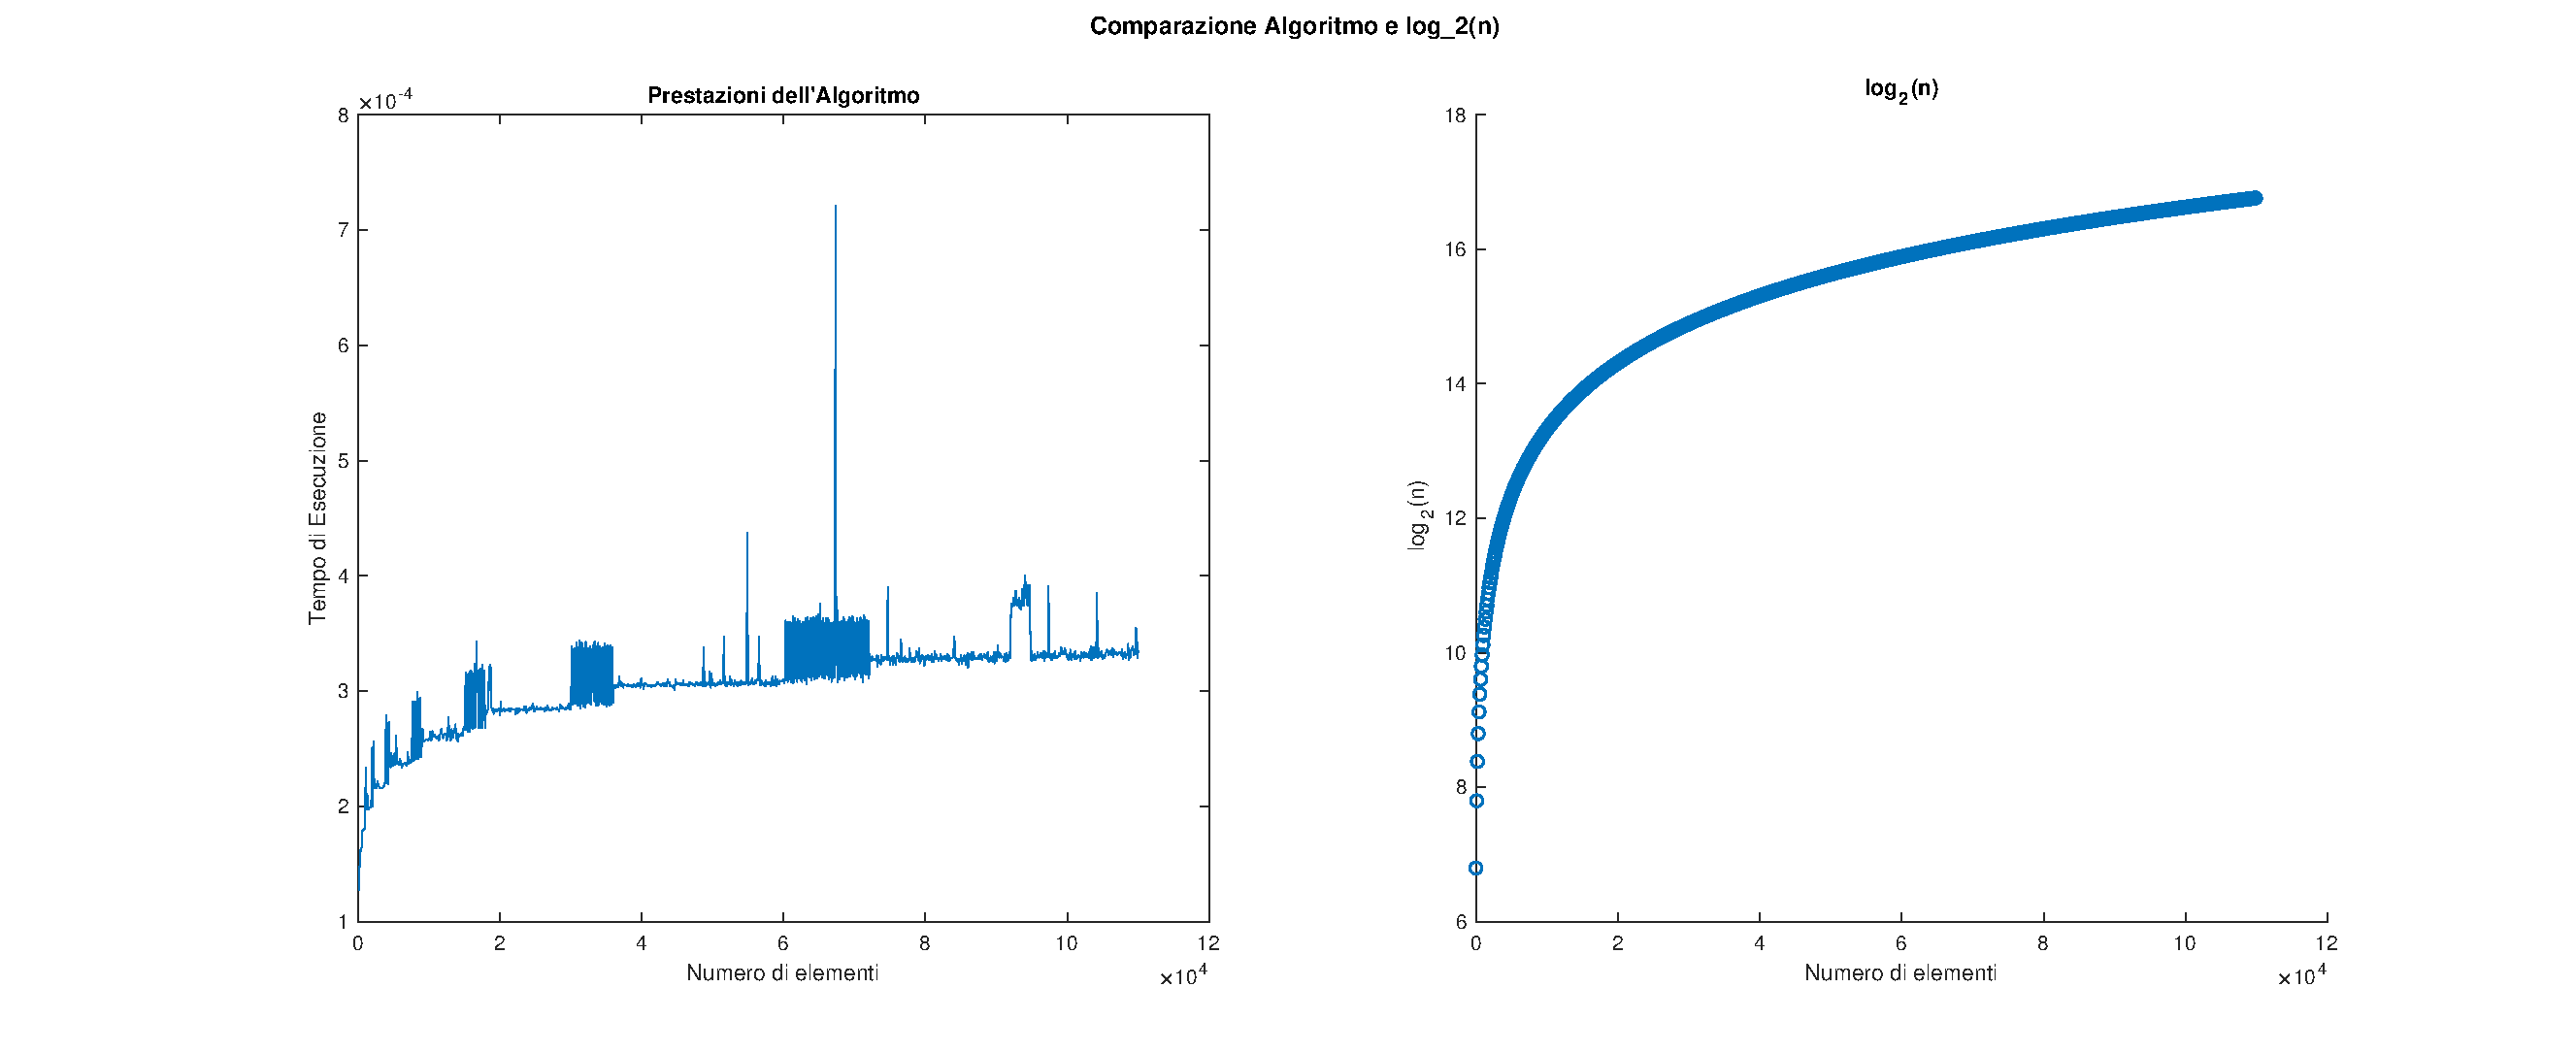
\includegraphics[width=\textwidth,height=\textheight,keepaspectratio]{./TeX_files/chart/comparison}
    \caption{Grafico che mette a confronto numero di elementi/tempo di esecuzione e  numero di elementi/$log_2$(\#elementi)}
\vspace{-10pt}
\end{figure}


\chapter{Conclusione}
\section{Riflessioni Finali}
L'interezza dell'algoritmo è stata così presentata in questa "breve" relazione. Al fine di aiutare nella comprensione del codice e della relazione stessa ho scritto effettivamente alcune funzioni sovrabbondati rispetto al codice fornitoci dai tutor, magari sprecato memoria nella creazione di un albero temporaneo od omesso alcuni passaggi di secondaria importanza dell'algoritmo in questa stessa relazione, tali scelte però sono state dettate da una criterio puramente "didattico" per aiutare nella migliore comprensione del codice.
Tutto il codice è rilasciato sotto la MIT License. 
\begin{flushright}
	\emph{Matteo Esposito}
\end{flushright}
%--------------------------------------%

\backmatter
\end{document}